\section{问题提出的背景}
计算机视觉是计算机科学的一个重要分支,它的核心任务是通过计算机对图像或视频进行理解,使计算机可以像人类的大脑一样对图像信息进行处理和解释,最终能够达到像人类一样通过视觉来观察和理解世界。其中,人是自然界中的十分重要的一类物体,对图像上的人体的分析也是计算机视觉领域的重要课题之一,吸引了国内外众多研究者的关注。

对人体的姿态分析的研究核心是从单张图片或者视频序列中检测、跟踪人体,获取人体的运动数据,并在此基础上重建人体的三维运动,更进一步能够描述和理解人体的行为。对于人类来说,看一张图片或一段视频,可以比较容易地理解其中的人体运动,但是对计算机来说,分析其姿态有许多困难:使用的人体模型不足以描述人体的运动;人体存在许多自遮挡或被外界物体遮挡,难以进行检测;图片中的信息是二维的,存在空间姿态上的歧义性;相机的参数有时难以获得,因此无法得到尺度信息;近些年计算机视觉领域在这个方向上进行了积极的探索,取得了许多重大的进展,然而距离实用还有一段距离。

\subsection{主要面临的困难}
目前,从视频序列或图片中恢复人体运动姿态和三维结构仍然存在许多困难,主要困难有以下:

\textbf{人体结构:}
人体是一个非刚体结构,自由度较多,并且人体的运动较为复杂,有高度的非线性特点。此外人体外表由于穿着不同的服装,对服装难以使用统一的模型加以表达。因此对人体姿态分析的研究工作需要从不同的角度入手,采用不同的约束条件来简化人体的结构描述。

\textbf{人体分割:}
从图片中检测以及分割出人体是一个困难但很重要的问题,由于环境中获取的图片受到许多方面的影响,比如天气、光照的变化,不同的背景的干扰,物体与环境之间以及物体与物体之间的遮挡等都给有效的运动分割带来了困难。
\begin{figure}[ht]
    \centering
    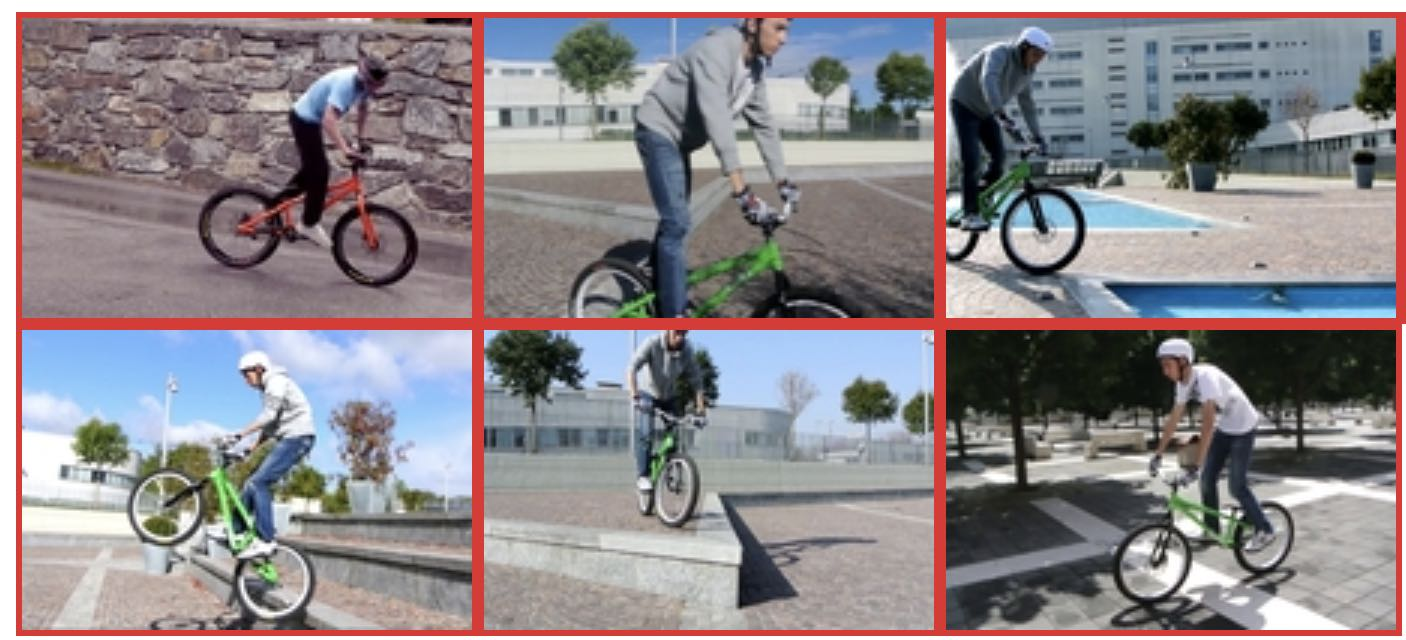
\includegraphics[height=.25\linewidth]{background/cha1}
    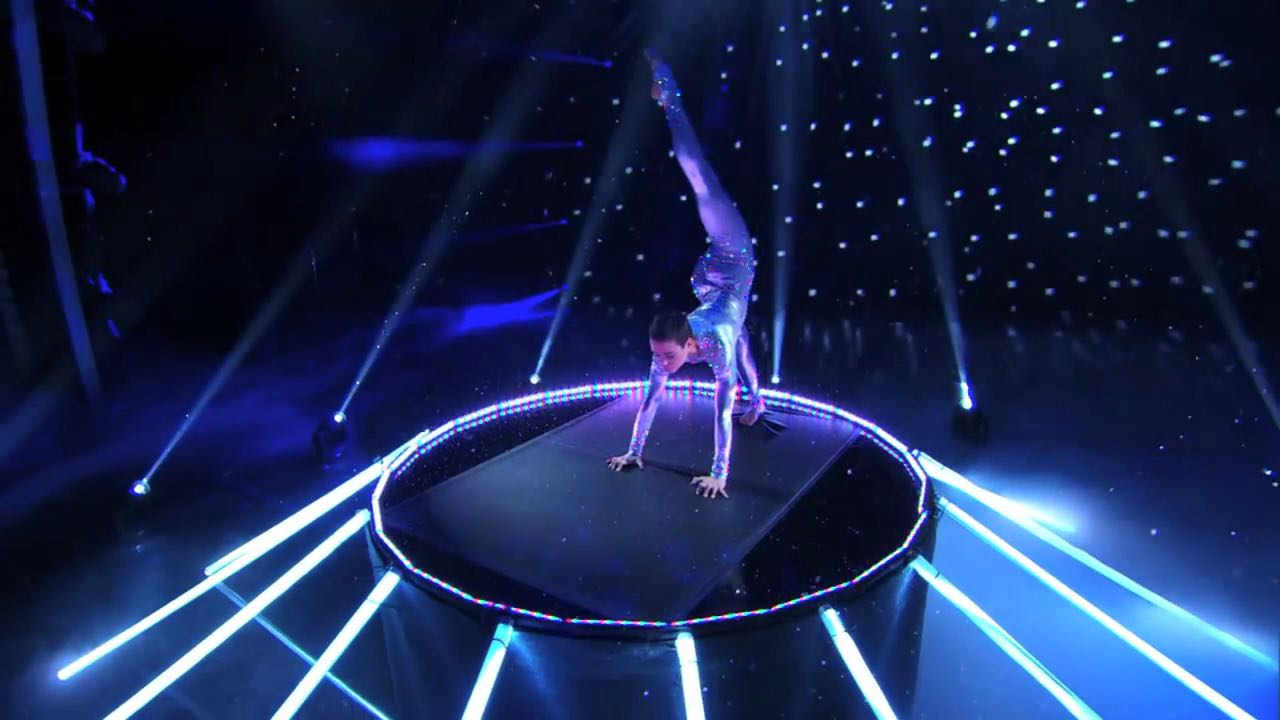
\includegraphics[height=.25\linewidth]{background/cha2}
    \caption{\label{fig:cha2}面临的挑战:外观、姿势、光照的差异}
\end{figure}

\textbf{对于任意视频的摄像机标定:}
在传统的计算机视觉领域中,对于计算机进行标定是必不可少的步骤。在基于视频的人体运动重构中,传统的方法需要采样步骤繁琐的摄像机标定,这限制了视频的来源。因此传统的方法只能对特定采集的视频进行处理,不能处理任意给定的视频,这限制了重建方法的应用范围。

\textbf{从三维到二维的深度歧义性:}
三维空间的物体投影到二维图像会丢失深度信息,而使用单个相机获取的视频去推导人体的三维动作属于病态(ill-posed)问题。从图像反向映射到空间不是唯一的,因此这种深度的歧义性使得人体的三维运动的获取变得极为困难。
